\documentclass[a4paper, 14pt]{report}
\usepackage{extsizes}
\usepackage[T2A]{fontenc}
\usepackage[utf8]{inputenc}
\usepackage[english,russian]{babel}
\usepackage{amssymb,amsfonts,amsmath,mathtext,cite,enumerate,float}
\usepackage[dvips]{graphicx}
\usepackage{indentfirst}

\graphicspath{{../img/}}

\usepackage{geometry}
\geometry{left=2cm}
\geometry{right=1.5cm}
\geometry{top=1cm}
\geometry{bottom=2cm}

\usepackage[T1]{fontenc}
\usepackage{titlesec, blindtext, color}
\definecolor{gray75}{gray}{0.75}
\newcommand{\hsp}{\hspace{20pt}}
\titleformat{\chapter}[hang]{\Huge\bfseries}{}{0pt}{\Huge\bfseries}

\renewcommand{\theenumi}{\arabic{enumi}}
\renewcommand{\labelenumi}{\arabic{enumi}}
\renewcommand{\theenumii}{.\arabic{enumii}}
\renewcommand{\labelenumii}{\arabic{enumi}.\arabic{enumii}.}
\renewcommand{\theenumiii}{.\arabic{enumiii}}
\renewcommand{\labelenumiii}{\arabic{enumi}.\arabic{enumii}.\arabic{enumiii}.}

\usepackage{setspace}
\onehalfspacing

\bibliographystyle{unsrt}
\renewcommand{\labelitemi}{--}

\usepackage{subcaption}

\usepackage{amsthm}
\makeatletter
\renewcommand*{\thetable}{\arabic{table}}
\renewcommand*{\thefigure}{\arabic{figure}}
\let\c@table\c@figure
\let\ftype@table\ftype@figure
\def\@endtheorem{$\qed$}
%\renewcommand\@endtheorem{\vvv@endmarker\endtrivlist\@endpefalse}
\makeatother

\theoremstyle{definition}
\newtheorem*{definition}{Определение}
\newtheorem*{note}{Замечание}
\newtheorem*{example}{Пример}
\newtheorem*{theorem}{Теорема}
\newtheorem*{implication}{Следствие}

\usepackage{subcaption}

\begin{document}
	
\tableofcontents
\chapter{Двойной интеграл}	
	\section{Площадь плоской фигуры.}
		Пусть $D$ - фигура на плоскости. Что есть площадь? Если $D$ - треугольник, прямоугольник, многоугольник, то площадь вводится естественным образом.
		\begin{figure}[!htp]
			\centering
			\begin{subfigure}{0.20\linewidth}
				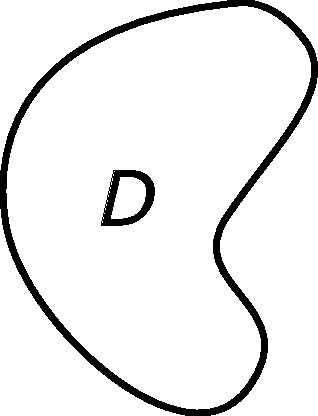
\includegraphics[width=1\linewidth]{sampleD}
				\caption{}
				\label{fig:area_d}
			\end{subfigure}
			\hfill
			\begin{subfigure}{0.20\linewidth}
				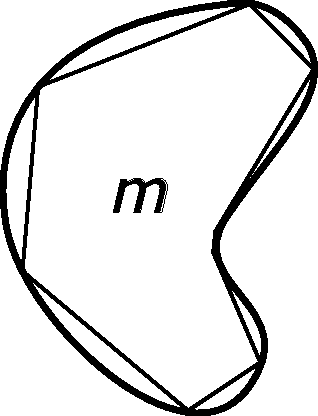
\includegraphics[width=1\linewidth]{sampleD_smM}
				\caption{}
				\label{fig:area_d_inner_m}
			\end{subfigure}
			\hfill
			\begin{subfigure}{0.20\linewidth}
				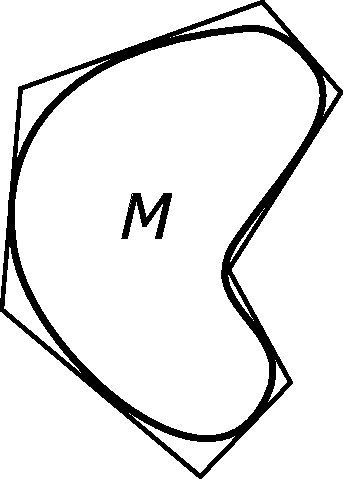
\includegraphics[width=1\linewidth]{sampleD_bigM}
				\caption{}
				\label{fig:area_d_outer_m}
			\end{subfigure}
			\caption{Область $D$}
		\end{figure}
		
		\begin{enumerate}
			\item Рассмотрим множество многоугольников $m$, целиком содержащихся в $D$
			(рисунок \ref{fig:area_d_inner_m}).
			$S(m)$ - площадь $m$
			
			\item Рассмотрим множество многоугольников $M$, целиком содержащихся в $D$
			(рисунок \ref{fig:area_d_outer_m}).
			$S(M)$ - площадь $M$
		\end{enumerate}
	
		\begin{definition}
			Область $D$ на плоскости, называется квадрируемой, если выполняются следующие условия:
			\begin{enumerate}
				\item $\exists S_*=\sup S(m)$
				\item $\exists S^*=\inf S(M)$
				\item $S_*=S^*$
			\end{enumerate}
		
			При этом величина $S=S_*=S^*$ называется площадью квадрируемой области $D$
		\end{definition}
	
		\begin{definition}
			Говорят, что множество $D$ точек плоскости имеет площадь 0, если $D$ можно заключить в многоугольник сколь угодно малой площади, то есть
			\begin{equation}
				\forall\epsilon>0~\exists\text{многоугольник }M:(D\subseteq M) \& (S(M)<\epsilon)
			\end{equation}
		\end{definition}		
	
		\begin{example}
			К множествам точек с нулевой плоскостью относятся:
			\begin{enumerate}
				\item точка (рисунок \ref{fig:zero_s_dot})
				\item отрезок (рисунок \ref{fig:zero_s_segment})
				\item гладкая кривая (рисунок \ref{fig:zero_s_curve})
			\end{enumerate}
		
			\begin{figure}[!h]
				\centering
				\begin{subfigure}{0.20\linewidth}
					\centering
					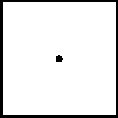
\includegraphics[width=1\linewidth]{zeroS_dot}
					\caption{}
					\label{fig:zero_s_dot}
				\end{subfigure}
				\hfill
				\begin{subfigure}{0.30\linewidth}
					\centering
					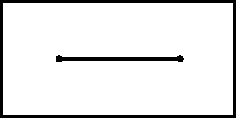
\includegraphics[width=1\linewidth]{zeroS_segment}
					\caption{}
					\label{fig:zero_s_segment}
				\end{subfigure}
				\hfill
				\begin{subfigure}{0.35\linewidth}
					\centering
					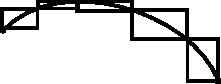
\includegraphics[width=1\linewidth]{zeroS_curve}
					\caption{}
					\label{fig:zero_s_curve}
				\end{subfigure}
				\caption{Множества точек плоскости с нулевой площадью}
			\end{figure}
		\end{example}
		
		\begin{theorem}
			Пусть $D$ -- замкнутая область. Тогда $D$ -- квадрируема тогда и только тогда, когда граница $D$ имеет нулевую площадь.
		\end{theorem}
		\begin{theorem}
			Пусть $L$ -- плоская кривая конечной длины. Тогда $L$ имеет площадь нуль.
		\end{theorem}
		\begin{implication}
			Если $D$ -- плоская область, ограниченная конечным набором гладких кривых, каждая из которых имеет конечную длину, то $D$ -- квадрируема.
		\end{implication}
		\begin{note}
			В дальнейшем, если иное не оговорено, будем рассматривать только квадрируемые области.
		\end{note}
		
	\section{Задачи, приводящие к понятию двойного интеграла}
		\subsection{Задача об объёме цилиндрического тела}
			Пусть:
			\begin{enumerate}
				\item $D$ - область на плоскости $xOy$
				\item $f:D\rightarrow R$
				\item $f(x,y)\ge0, (x,y)\in D$
			\end{enumerate}
		
			Рассмотрим тело:
			\begin{equation}
				T=\{
					(x,y,z): 
					(x,y)\in D,~
					0\le z\le f(x,y)
				\}
			\end{equation}
		
			\begin{figure}[!ht]
				\centering
				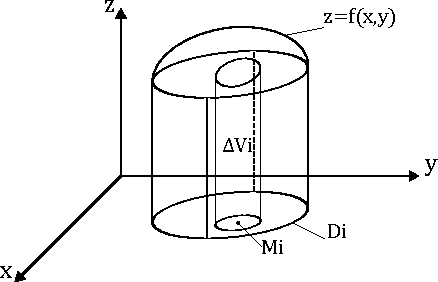
\includegraphics[width=0.5\linewidth]{body_t}
				\caption{Тело $T$}
				\label{fig:body_t}
			\end{figure}
		
			Найдём объём тела $T$.
			\begin{enumerate}
				\item Раздробим область $D$ на части
					\begin{equation}
						D=\bigcup_{i=\overline{1,n}}D_i\text{; где }intD_i\cap intD_j=\emptyset, i\ne j
					\end{equation}
					$intD$ - множество внутренних точек области $D$. Важно отметить, что она должна быть разделена без пересечений, как на рисунке \ref{fig:area_d_intersect}, но допустимо наличие границы, как на рисунке \ref{fig:area_d_no_intersect}
					\begin{figure}[!ht]					
						\begin{subfigure}{0.40\linewidth}
							\centering
							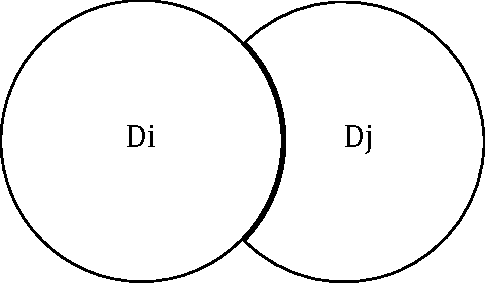
\includegraphics[width=1\linewidth]{area_d_no_intersect}
							\caption{}
							\label{fig:area_d_no_intersect}
						\end{subfigure}
						\hfill
						\begin{subfigure}{0.5\linewidth}
							\centering
							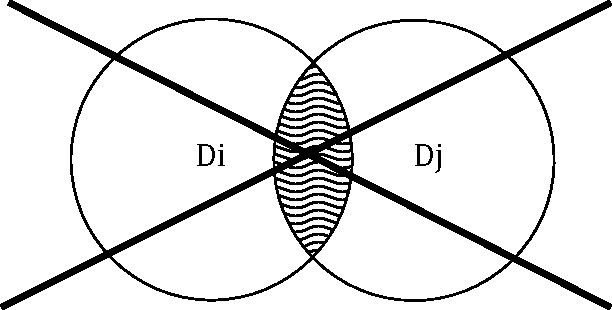
\includegraphics[width=1\linewidth]{area_d_intersect}
							\caption{}
							\label{fig:area_d_intersect}
						\end{subfigure}
					\caption{}
					\end{figure}
			
				\item Выберем в каждой из $D_i, i=\overline{1,n}$ точку $M_i\in D$
				\item Объём $\Delta V_i$ той части тела $T$, которая расположена над $D_i$, рассчитывается по формуле:
					\begin{equation}
						\Delta V_i\approx f_i\cdot S(D_i); ~f_i=f(M_i)
					\end{equation}
					Считаем, что размеры $D_i$ малы, тогда объём $\Delta V$ приближённо равен объёму цилиндра, высота которого $f(M_i)$, а площадь основания $S(D_i)$. Обозначим $\Delta S_i=S_i(D_i), ~i=\overline{1,n}$

				\item Объём всего тела $T$:
					\begin{equation}
						V(T)=\sum_{i=1}^{n}\Delta V_i\approx\sum_{i=1}^{n}f_i\Delta S_i
					\end{equation}
			\end{enumerate}
		
			\begin{definition}
				Диаметром области $D$ называется число:
				\begin{equation}
					diamD=\sup|MN|; ~M,N\in D
				\end{equation}
			\end{definition}
		
		\subsection{Задача о массе пластины}
			Пусть пластина занимает плоскую область $D$ на плоскости $Oxy$, $f(x,y)\ge0$ - значение поверхностной плотности материала в точке $(x,y)\in D$. Как найти массу $m(D)$ пластины? Данная задача решается точно так-же, как и предыдущая, потому разбирать повторно мы её не будем.
	
	\section{Определение двойного интеграла}
		\subsection{Двойной интеграл единицы}
			Пусть $D$ - квадрируемая замкнутая область на $Oxy$.
			\begin{definition}
				Разбиением области $D$ будет называться множество
				\begin{equation}
					R=\{D_1,D_2,...,D_n\},
				\end{equation}
				где $D_i\le D, i=\overline{1,n};
				~D=\bigcup D_i;
				~intD_i\cap intD_j\ne\emptyset, i\ne j$
			\end{definition}
		
			\begin{definition}
				Диаметром разбиения $R$ на число $d(R)=\underset{i=\overline{1,n}}{\max}(diamD_i)$
			\end{definition}
		
			Пусть $f:D\rightarrow R$ - заданная в области $D$ функция двух переменных (не обязательно $f\ge 0$)
			\begin{definition}
				Двойным интегралом функции $f$ по области $D$ называется число
				\begin{equation}
					\iint\limits_{D}f(x,y)dxdy=\lim_{d(R)\rightarrow0}\sum_{i=1}^{n}f(M_i)\Delta S_i,
				\end{equation}
				где $\Delta S_i=S(D_i),~
				M_i\in D,~
				i=\overline{1,n},~
				R=\{D_1,D_2,...,D_n\}$ -- разбиение обл. $D$
			\end{definition}
		
			\begin{note}
				В определении подразумевается, что указанный предел существует, конечен и не зависит от способа выбора точек $M_i\in D_i$, а так же от способа разбиения области $D$.
			\end{note}
		
			\begin{definition}
				Функция $f$, для которой $\exists\iint\limits_{D}fdxdy$, называется интегрируемой в области $D$.
			\end{definition}
	\section{Свойства двойного интеграла}
		\subsection{Двойной интеграл единицы}		
			Если $D$ имеет конечную площадь $S(D)$, то
			\begin{equation}
				\iint\limits_{D}1dxdy=S(D)
			\end{equation}
		\subsection{Линейность}
			Если $f$, $g$ интегрируемы в $D$, то функция $f\pm g$ тоже интегрируема в $D$, причём:
			\begin{equation}
				\iint\limits_{D}(f\pm g)dxdy=\iint\limits_{D}fdxdy\pm\iint\limits_{D}dxdy
			\end{equation}
			
			Если $f$ интегрируема в $D$, то $c\cdot f, c = const$ тоже интегрируема в $D$, причём:
			\begin{equation}
				\iint\limits_{D}(c\cdot f)dxdy=c\cdot\iint\limits_{D}fdxdy
			\end{equation}
		\subsection{Аддитивность}
			Пусть $f$ интегрируема в $D_1$ и $D_2$ и $intD_1\cap intD_2=\emptyset$. Тогда $f$ интегрируема в $D_1\cup D_2$, причём:
			\begin{equation}
				\iint\limits_{D_1\cup D_2}fdxdy=\iint\limits_{D_1}fdxdy+\iint\limits_{D_2}fdxdy
			\end{equation}
		\subsection{О сохранении интегралом знака функции}
			Пусть $f(x,y)\ge0$ в $D$ и $f$ интегрируема в $D$. Тогда:
			\begin{equation}
				\iint\limits_{D}fdxdy\ge0
			\end{equation}
		\subsection{О сохранении интегралом неравенства подынтегральных функций}
			Пусть $f(x, y)\ge g(x, y)$ в $D$ и $f, g$ интегрируемы в $D$. Тогда:
			\begin{equation}
				\iint\limits_{D}fdxdy\ge \iint\limits_{D}gdxdy
			\end{equation}
		\subsection{Теорема об оценке модуля двойного интеграла}
			Пусть $f$ интегрируема в $D$. Тогда $|f|$ тоже интегрируема в $D$, причём:
			\begin{equation}
				\left|\iint\limits_{D}fdxdy\right|\ge\iint\limits_{D}fdxdy
			\end{equation}
		\subsection{Теорема об оценке двойного интеграла}
			Пусть $f$ и $g$ интегрируемы в $D$, $m\le f\le M$ в $D$, $g(x,y)\ge0$ в $D$. Тогда:
			\begin{equation}
				m\iint\limits_{D}gdxdy\le\iint\limits_{D}(f\cdot g)dxdy\le M\iint\limits_{D}gdxdy
			\end{equation}

			\begin{implication}
				При $g(x,y)=1$ в $D$, имеет место:
				\begin{equation}
					m\cdot S(D)\le\iint\limits_{D}fdxdy\le M\cdot S(D)
				\end{equation}
			\end{implication}
		\subsection{Теорема о среднем значении для двойного интеграла}\label{subsec:theorem_of_average}
			Пусть $D$ -- линейно-связная, квадрируемая замкнутая область, $f$ -- непрерывна и интегрируема в $D$. Тогда $\exists$ точка $M_0(x_0, y_0)\in D$ такая, что
			\begin{equation}
				f(M_0)=\frac{1}{S(D)}\iint_{D}f(x, y)dxdy
			\end{equation}
			
			Замечание: правую часть формули из свойства 8 называют среднем значением функции $f$ в области $D$
			
			\begin{definition}
				Область называется линейно-связной, если её граница является связным множеством.
			\end{definition}
			
			\begin{definition}
				Множество $O$ называется связным, если $\forall$ точек $M_1, M_2 \exists$ кривая $S\in O$
			\end{definition}
		\subsection{Обобщённая теорема о среднем}
			Пусть:
			\begin{enumerate}
				\item $f$ - непрерывна на $D$
				\item $g$ - интегрируема на $D$
				\item $g$ - знакопостоянна на $D$
				\item $D$ - линейно связная область
			\end{enumerate}
			
			Тогда $\exists M_o\in D$ такая, что
			\begin{equation}
				\iint\limits_{D}f(x,y)g(x,y)dxdy=f(M_0)\iint\limits_{D}g(x,y)dxdy
			\end{equation}
		
			\begin{note}
				При $g(x,y)=1$, свойство $g$ совпадает с свойством \ref{subsec:theorem_of_average}.
			\end{note}
	\section{Вычисление двойного интеграла}
		Пусть $D$ - область на плоскости $Oxy$. По определению $D$ называется y-правильной, если её можно задать в виде:
		\begin{equation}
			\label{eq:y_right}
			D=\{(x, y): a \le x \le b, \phi_2(x)\le y\le\phi_2(x)\}
		\end{equation}
		
		\begin{note}
			Область $D$ является y-правильной тогда и только тогда, когда любая прямая параллельная плоскости $Oxy$ пересекает границу $D$ не более чем в двух точках, либо содержит участок границы целиком.
		\end{note}
		
		\begin{figure}[!ht]
			\centering
			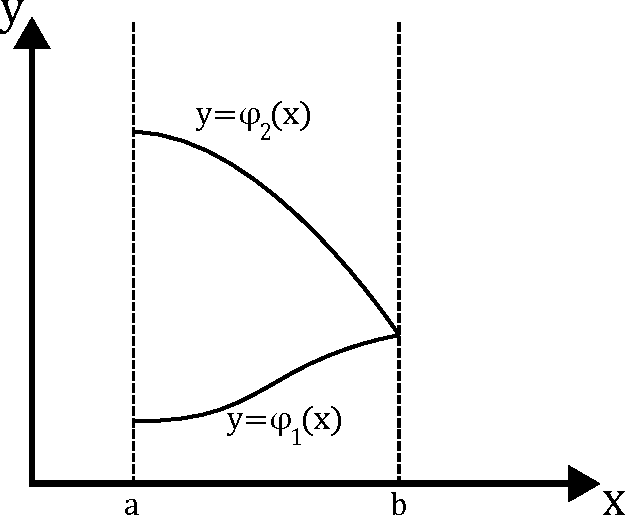
\includegraphics{y_right}
			\caption{}
			\label{fig:y_right}
		\end{figure}
		
		\begin{theorem}
			Пусть:
			\begin{enumerate}
				\item $\exists\iint\limits_D f(x, y)dxdy=I$
				\item $D$ является y-правильной и удовлетворяет формуле \ref{eq:y_right}
				\item $\forall x\in[a,b]~\exists F(x)=\int\limits_{\phi_1(x)}^{\phi_2(x)}f(x,y)dy$
			\end{enumerate}
			
			Тогда существует повторный интеграл
			\begin{equation}
				I_{\text{повт.}}
				=\int\limits_a^bdx \int\limits_{\phi_1(x)}^{\phi_2(x)}f(x,y)dy
				=\int\limits_a^bF(x)dx
				=I
			\end{equation}
		\end{theorem}
		
		\begin{note}
			Область называется x-правильной, если её можно задать в виде:
			\begin{equation}
				\label{eq:x_right}
				D=\{(x,y):c\le y\le d,\phi_1(y)\le x\le \phi_2(y)\}
			\end{equation}
			
			Пусть:
			\begin{enumerate}
				\item $\exists\iint\limits_D f(x, y)dxdy=I$
				\item $D$ является x-правильной и удовлетворяет формуле \ref{eq:x_right}
				\item $\forall y\in[c,d]\exists F(y)=\int\limits_{\phi_1(y)}^{\phi_2(y)}f(x,y)dx$
			\end{enumerate}
		
			Тогда:
			\begin{equation}
				\iint\limits_Df(x,y)dxdy=\int\limits_c^ddy\int\limits_{\phi_1(y)}^{\phi_2(y)}f(x,y)dx
			\end{equation}
		\end{note}
	
		Если область $D$ не является правильной в направлении какой-либо координатной оси (как представлено на рисунке \ref{fig:unreal_hardcore_d}, то её можно разбить на правильные части и использовать свойство аддитивности двойного интеграла.
		
	\section{Замена переменных в двойном интеграле}
		Замена переменных позволяет сложные ситуации (как на рисунке \ref{fig:unreal_hardcore_d}) преобразовывать к более простым (рис. \ref{fig:easy_af_d}).
		\begin{figure}[!ht]
			\begin{subfigure}{0.4\linewidth}
				\centering
				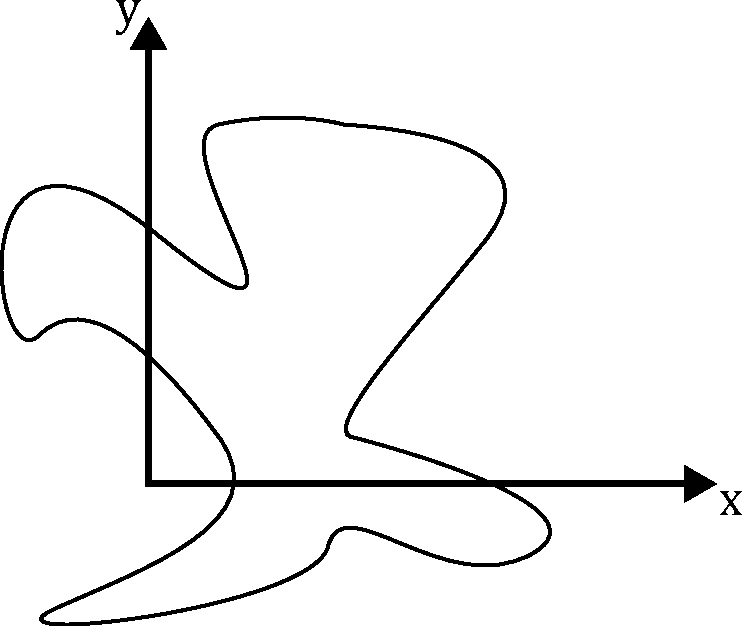
\includegraphics[width=1\linewidth]{hardcore_d}
				\caption{}
				\label{fig:unreal_hardcore_d}
			\end{subfigure}
			\hfill
			\begin{subfigure}{0.4\linewidth}
				\centering
				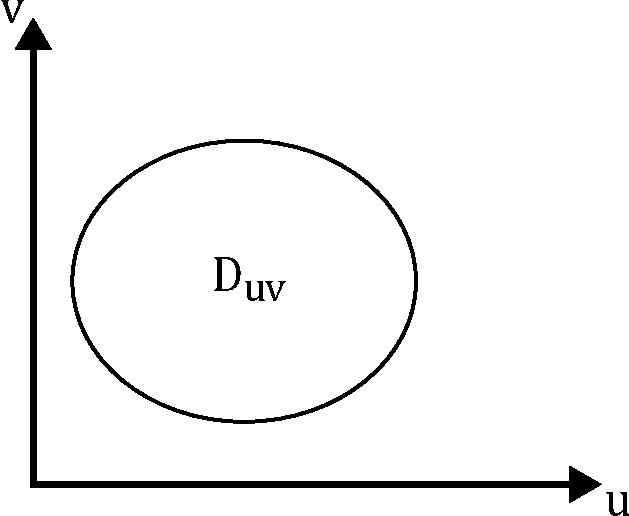
\includegraphics[width=1\linewidth]{easy_af_d}
				\caption{}
				\label{fig:easy_af_d}
			\end{subfigure}
			\caption{}
		\end{figure}
	
		Пусть $I=\iint\limits_{D_{xy}}f(x,y)dxdy$. Предположим подобрано преобразование:
	 	\begin{subequations}
	 		\begin{align}
	 			\Phi&:D_{uv}\rightarrow D_{xy} \\
		 		\Phi&:\begin{cases}
		 			x=x(u,v) \\
		 			y=y(u,v)
		 		\end{cases}
	 		\end{align}
	 	\end{subequations}
 	
 	 	\begin{theorem}[О замене переменных в двойном интеграле]
 	 		Пусть:
		 	\begin{enumerate}
				\item $D_{xy}=\Phi(D_{uv})$
		 		\item $\Phi$ - биекция. 
		 		\item $\Phi$ - непрерывна и параллельна диаграмме.
		 		\item Якобиан отображения к $\Phi$:
		 		\begin{equation}
		 			J_\Phi=\begin{vmatrix}
		 				x'_u & x'_v \\
		 				y'_u & y'_v
		 			\end{vmatrix}\ne0\text{ в }D_{uv}
		 		\end{equation}
		 		\item $f$ интегрируема в $D_{xy}$
			\end{enumerate}
		 		
			Тогда справедливо:
			\begin{equation}
				\iint\limits_{D_{xy}}f(x,y)dxdy
				=\iint\limits_{D_{uv}}
					f(x(u,v),y(u,v))
					|J_\Phi(u,v)|
				dudv
			\end{equation}
		\end{theorem}
	
 		\begin{note}
 			Аналогия с обычным интегралом:
 			\begin{equation}
 				\int\limits_a^bf(x)dx=
 				\begin{vmatrix}
 					x=\xi(t) \\
 					dx=\xi'(t)dt \\
 					x=a\Rightarrow t=\xi^{-1}(a) \\
 					x=b\Rightarrow t=\xi^{-1}(b)
 				\end{vmatrix}
					=\int\limits_{\xi^{-1}(a)}^{\xi^{-1}(b)}f(\xi(t))\xi'(t)dt
 			\end{equation}
 		\end{note}
 	
 		\begin{note}
		 	Теорема останется справедливой и в случае, когда свойства 2, 3, 4 нарушаются в отдельных точках области $D$ или на конечном числе кривых площади 0.
	 	\end{note}
		
		\begin{example}
			Переход в двойном интеграле к полярным координатам. В прямоугольная декартова система состоит из начала координат и двух взаимно перпендикулярных осей. Положение точки в такой системе задаётся с помощью пары чисел $(x, y)$, геометрическая интерпретация которых такова: первое число $x$ есть проекция точки на ось $X$, второе число $y$ есть проекция точки на ось $Y$.
			
			Полярная система координат состоит из начала координат O и луча P. Каждая точка задаётся как пара чисел $(\rho, \phi)$. $\rho$ задаёт расстояние на луче P, $\phi$ задаёт угол против часовой стрелки, на который нужно повернуть получившийся радиус-вектор, чтобы достичь точки $M$
			
	 		Связь полярной системы координат с декартовой:
	 		\begin{equation}
	 			\begin{cases}
	 				x=\rho \cos(\phi)\\
	 				y=\rho \sin(\phi)
	 			\end{cases}
 				~
 				J_\Phi(\rho, \phi)=
 				\begin{vmatrix}
 					x'_\rho & x'_\phi \\
 					y'_\rho & y'_\phi
 				\end{vmatrix}=
	 			\begin{vmatrix}
	 				\cos\phi & -\rho\sin\phi \\
	 				\sin\phi & \rho\cos\phi
	 			\end{vmatrix}=
 				\rho\cos^2\phi+\rho\sin^2\phi=\rho
	 		\end{equation}
 			
 			Таким образом:
 			\begin{equation}
 				\iint\limits_{D_{xy}}f(x,y)dxdy=
 				\iint\limits_{D_{\rho\phi}}f(x\cos\phi, y\sin\phi)\rho d\rho d\phi
 			\end{equation}
	 	\end{example}
 	
 	\section{Приложения двойного интеграла}
 		\subsection{Вычисления площади плоской фигуры}
 			\begin{equation}
 				S(D)=\iint\limits_{D}1dxdy
 			\end{equation}
 		
 		\subsection{Вычисление массы пластины}
 			Пусть $f(x,y)$ - значение поверхностной плотности. Тогда масса пластины:
 			\begin{equation}
 				m=\iint\limits_{D}f(x,y)dxdy
 			\end{equation}
 		
 		\subsection{Вычисление координат центра тяжести}
 			Пусть $f(x,y)$ - значение поверхностной плотности. $(x_0,y_0)$ -- координаты центра тяжести.
 			\begin{subequations}
 				\begin{align}
 					x_0=\frac{1}{m(D)}\iint\limits_{D}xf(x, y)dxdy \\
 					y_0=\frac{1}{m(D)}\iint\limits_{D}yf(x, y)dxdy
 				\end{align}
 			\end{subequations}
 		
 		\subsection{Вычисление объёма тела}
	 		\begin{subequations}
	 			\begin{align}
	 				T&=\{(x,y,z): x,y\le D_{xy},z_1(x,y)\le z\le z_2(x,y)\} \\
	 				V(T)&=\iint\limits_{D_{xy}}[z_2(x,y)-z_1(x,y)]dxdy
	 			\end{align}
	 		\end{subequations}
 			
\chapter{Теория вероятностей}
	\section{Определение вероятности}
		\subsection{Случайный эксперимент}
			Случайным называется такой эксперимент, результат которого невозможно точно предсказать.
			
			\begin{example}[1]
				Бросают монету. Возможные результаты - выпадение орла или решки
				\begin{equation}
					\Omega=\{O, P\}
				\end{equation}
			\end{example}
					
			\begin{example}[2]
				Бросают шестигранную игральную кость.
				
				\begin{equation}
					\Omega=\{1, 2, 3, 4, 5, 6\}
				\end{equation}
			\end{example}
				
			\begin{example}[3]
				Из колоды из 36 карт извлекают две карты
				\begin{equation}
					\label{eq:cards}
					\Omega=\{(x_1, x_2): x_i\text{ - номер карты, которую достали при извлечении}\}
				\end{equation}
				В данном случае, число возможных исходов равно $36\cdot 35=1260$. Можно записать уравнение \ref{eq:cards} следующим образом:
				\begin{equation}
					\Omega=\{(x_1, x_2): x_i\in {1,...,36}, x_1\ne x_2\}
				\end{equation}
			\end{example}
				
			\begin{example}[4]
				Бросают монету, до первого появления решки. 
				\begin{equation}
					\Omega=\{1,2,3,...\}, |\Omega|=\aleph_0
				\end{equation}
			\end{example}
				
			\begin{example}[5]
				Производят выстрел по плоской мишени. Возможный исход описывается парой $(x_1,x_2)$.
				\begin{equation}
					\Omega=\{(x_1, x_2): x_1\in\mathbb{R},x_2\in\mathbb{R}\}
				\end{equation}
			\end{example}
		
			\begin{definition}
				Множеством всех возможных исходов случайного эксперимента называется множество всех возможных элементарных исходов.
			\end{definition}
			
			\begin{note}
				В этом определении предполагается, что:
				\begin{enumerate}
					\item каждый исход из $\Omega$ является делимым и неделимым, то есть не может быть разбит на более мелкие исходы в рамках данного эксперимента
					\item в результате проведения эксперимента, обязательно имеет место ровно один элементарный исход
				\end{enumerate}
			\end{note}
		
			\begin{definition}[нестрогое]
				Событием (или, более точно, случайным событием) называется любое подмножество множества $\Omega$ элементарных исходов.
			\end{definition}
			
			\begin{definition}
				Говорят, что в результате эксперимента произошло событие $A$, если наступил один из входящих в $A$ исходов.
			\end{definition}
			
			РИСУНОК
			
			\begin{definition}
				Говорят, что событие $A$ является следствием события $B$, если наступление события $B$ всегда влечёт наступление события $A$, то есть $B\subseteq A$
			\end{definition}
		
			\begin{figure}[!ht]
				\centering
				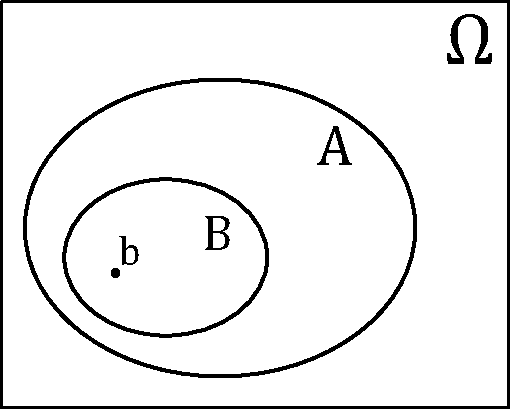
\includegraphics[width=0.3\linewidth]{probability_subsets}
				\caption{}
				\label{fig:probability_subsets}
			\end{figure}
			
			\begin{note}
				Любое множество $\Omega$ содержит подмножества $\emptyset$ и $\Omega$. Соответствующее событие считается невозможным $\emptyset$ и достоверным $\Omega$. Эти события называются несобственными, а все остальные -- собственными.
			\end{note}
			
			\begin{example}
				Из ящика, содержащего 2 красных и 3 синих шара, извлекают 1 шар.
				\begin{subequations}
					\begin{align}
						A&=\{\text{извлечённый шар красный или синий}\}=\Omega \\
						B&=\{\text{извлечённый шар белый}\}=\emptyset
					\end{align}
				\end{subequations}
			\end{example}
		
			\begin{definition}
				Событие (или случайное событие) - множество, являющееся подмножеством $\Omega$.
			\end{definition}
			
			Суммой событий $A$ и $B$ определено как:
			\begin{equation}
				A+B=A\cup B
			\end{equation}
		
			Произведение событий $A$ и $B$ определяется так:
			\begin{equation}
				A\cdot B=AB=A\cap B
			\end{equation}
			
			Событие, противоположное $A$ определено как:
			\begin{equation}
				\bar{A}=\Omega\setminus A
			\end{equation}
		
	\section{Свойства операций над событиями(основные)}
		\begin{enumerate}
			\item $A+B=B+A$
			\item $AB=BA$
			\item $(A+B)+C=A+(B+C)$
			\item $(AB)C=A(BC)$
			\item $A(B+C)=AB+AC$
			\item $A+BC=(A+B)(A+C)$
			\item $\bar{\bar{A}}=A$
			\item $A+A=A$
			\item $AA=A$
			\item $\bar{A+B}=\bar{A}\bar{B}$
			\item $\bar{AB}=\bar{A}+\bar{B}$
			\item $A\subseteq B\Leftrightarrow A+B=B$
			\item $A\subseteq B\Leftrightarrow AB=A$
			\item $A\subseteq B\Leftrightarrow \bar{A}\supseteq\bar{B}$
		\end{enumerate}
		
		Определения:
		\begin{enumerate}
			\item События $A$ и $B$ являются несовместными, если $A\cdot B=\emptyset$.
			\item События $A_1,...,A_n$ называются попарно несовместными, если любые два из них -- несовместные.
			\item События $A_1,...,A_n$ называются несовместными в совокупности, если\newline$A_1\cdot A_2\cdot...\cdot A_n=\emptyset$
		\end{enumerate}
		
		Очевидно, что если $A_1,...,A_n$ - попарно несовместны, то они несовместны в совокупности.
		
	\section{Классическое определение вероятности}
		Пусть $|\Omega|=N<\infty$, $A\subseteq\Omega; |A|=N_A$ и по условиям эксперимента нет объективных оснований предпочесть тот или иной исход остальным (все исходы равновозможны). Тогда вероятностью осуществления события $A$ называется число:
		\begin{equation}
			P\{A\}=\frac{N_A}{N}
		\end{equation}
	
		\begin{example}
			Два раза бросают шестигранную игральную кость. Событие $A=\{\text{сумма выпавших очком больше или равна 11}\}$. $P\{A\}=?$
			
			Решение: исходом будем считать пару $(x_1,x_2)$, где $x_i=\{1,2,3,4,5,6\}$ -- число, выпавшее на кости. $\Omega=\{(x_1,x_2): x_i=\{1,2,3,4,5,6\}\}; |\Omega|=N=36$.
			
			$|A|=?$; $A=\{(5, 6), (6, 5), (6, 6)\}\Rightarrow|A|=3$. Считаем все исходы из $\Omega$ равновозможными. Используя классическое определение вероятности, получим, что:
			\begin{equation}
				P\{A\}=\frac{N_A}{N}=\frac{3}{36}=\frac{1}{12}
			\end{equation}
		\end{example}
	
		\subsection{Свойства вероятности}
			\begin{enumerate}
				\item $P\{A\}\ge0$
				\item $P\{\Omega\}=1$
				\item Если $A, B$ - несовместные, то
				\begin{equation}
					P\{A+B\}=P\{A\}+P\{B\}
				\end{equation}
			\end{enumerate}
		
			Доказательства:
			\begin{enumerate}
				\item $P\{A\}=\frac{N_A}{N}\ge0$, что следует из $N_A\ge0, N\ge0$
				\item $P\{\Omega\}=\frac{N_\Omega}{N}=\{N(\Omega)=|\Omega|=N\}=\frac{N}{N}=1$
				\item $P\{A+B\}=\frac{N_{A+B}}{N} \\
				=\{N_{A+B}=|A+B|=|A|+|B|-|AB|=N_A+N_B\} \\
				=\frac{N_A+N_B}{N}=\frac{N_A}{N}+\frac{N_B}{N}=P\{A\}+P\{B\}$
			\end{enumerate}

	\section{Геометрическое определение вероятности}
		Геометрическое определение вероятности является обобщением классического на случай бесконечных элементарных исходов. Пусть выполнены следующие условия:
		\begin{enumerate}
			\item $\Omega\subseteq\mathbb{R}^n$
			\item $\mu(\Omega)<\infty$ - некая мера. 
				\subitem $\mu=1$ - длина
				\subitem $\mu=2$ - площадь
				\subitem $\mu=3$ - объём
				\subitem \dots
			\item возможность принадлежности исхода к тому или иному подмножеству $\Omega$ не зависит от формы события и его расположения внутри $\Omega$
		\end{enumerate}
	
		Тогда вероятность осуществления возможности события $A$ называется число $P\{A\} = \frac{\mu(N_A)}{\mu(N)}$
		
			\begin{example}
				Задача о встрече. Два человека договорились встретиться в условленном месте с 12:00 до 13:00. При этом, пришедший ждёт другого человека в течение 15 минут, а потом уходит. Какова вероятность того, что они встретятся, если появление каждого из них равновероятно в любое время в период с 12:00 до 13:00?
			
				Исход: $(x_1,x_2)$, где $x_i\in[0, 1]$; - время (в часах после 12:00) появления i-гоо человека в условленном месте. Тогда $\Omega=[0,1]\times[0,1]$.
				
				\begin{equation}
					A=\{(x_1, x_2): |x_1-x_2|\le \frac{1}{4}\}
				\end{equation}
				Используя геометрические определение, получаем:
				\begin{equation}
					P\{A\}
					=\frac{\mu(A)}{\mu(\Omega)}
					=\frac{\mu(\Omega)-2\cdot\mu(K)}{\mu(\Omega)}
					=\frac{1-2\cdot\frac{1\cdot3\cdot3}{2\cdot4\cdot4}}{1}
					=\frac{7}{16}
				\end{equation}
			
				\begin{figure}[!ht]
					\centering
					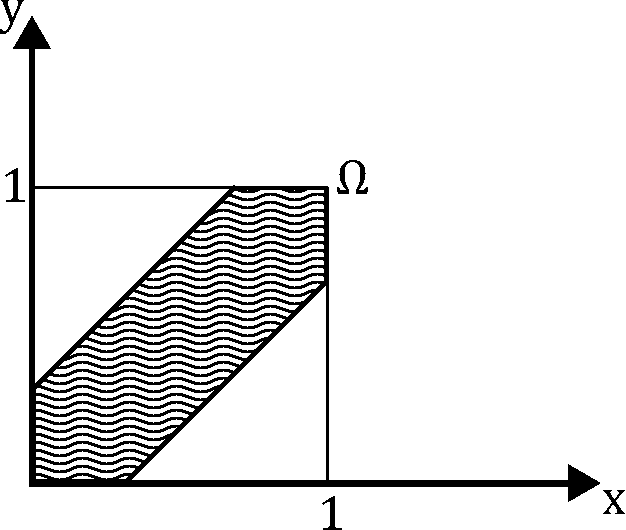
\includegraphics{2_jentleman_riddle}
					\caption{}
					\label{fig:2_jentleman_riddle}
				\end{figure}
			\end{example}
		
		
\end{document}